%%%%%%%%%%%%%%%%%%%%%%%%%%%%%%%%%%%%%%%%%
% Structured General Purpose Assignment
% LaTeX Template
%
% This template has been downloaded from:
% http://www.latextemplates.com
%
% Original author:
% Ted Pavlic (http://www.tedpavlic.com)
%
% Note:
% The \lipsum[#] commands throughout this template generate dummy text
% to fill the template out. These commands should all be removed when 
% writing assignment content.
%
%%%%%%%%%%%%%%%%%%%%%%%%%%%%%%%%%%%%%%%%%

%----------------------------------------------------------------------------------------
%   PACKAGES AND OTHER DOCUMENT CONFIGURATIONS
%----------------------------------------------------------------------------------------

\documentclass{article}

\usepackage{fancyhdr} % Required for custom headers
\usepackage{lastpage} % Required to determine the last page for the footer
\usepackage{extramarks} % Required for headers and footers
\usepackage{graphicx} % Required to insert images
\usepackage{lipsum} % Used for inserting dummy 'Lorem ipsum' text into the template
\usepackage{listings}
\usepackage{color}
\usepackage{amsmath}

\definecolor{dkgreen}{rgb}{0,0.6,0}
\definecolor{gray}{rgb}{0.5,0.5,0.5}
\definecolor{mauve}{rgb}{0.58,0,0.82}

\lstset{frame=tb,
  language=Python,
  aboveskip=3mm,
  belowskip=3mm,
  showstringspaces=false,
  columns=flexible,
  basicstyle={\small\ttfamily},
  numbers=none,
  numberstyle=\tiny\color{gray},
  keywordstyle=\color{blue},
  commentstyle=\color{dkgreen},
  stringstyle=\color{mauve},
  breaklines=true,
  breakatwhitespace=true
  tabsize=3
}

% Margins
\topmargin=-0.45in
\evensidemargin=0in
\oddsidemargin=0in
\textwidth=6.5in
\textheight=9.0in
\headsep=0.25in 

\linespread{1.1} % Line spacing

% Set up the header and footer
\pagestyle{fancy}
\lhead{\hmwkAuthorName} % Top left header
\chead{\hmwkClass\ (\hmwkClassInstructor\ \hmwkClassTime): \hmwkTitle} % Top center header
\rhead{\firstxmark} % Top right header
\lfoot{\lastxmark} % Bottom left footer
\cfoot{} % Bottom center footer
\rfoot{Page\ \thepage\ of\ \pageref{LastPage}} % Bottom right footer
\renewcommand\headrulewidth{0.4pt} % Size of the header rule
\renewcommand\footrulewidth{0.4pt} % Size of the footer rule

\setlength\parindent{0pt} % Removes all indentation from paragraphs

%----------------------------------------------------------------------------------------
%   DOCUMENT STRUCTURE COMMANDS
%   Skip this unless you know what you're doing
%----------------------------------------------------------------------------------------

% Header and footer for when a page split occurs within a problem environment
\newcommand{\enterProblemHeader}[1]{
\nobreak\extramarks{#1}{#1 continued on next page\ldots}\nobreak
\nobreak\extramarks{#1 (continued)}{#1 continued on next page\ldots}\nobreak
}

% Header and footer for when a page split occurs between problem environments
\newcommand{\exitProblemHeader}[1]{
\nobreak\extramarks{#1 (continued)}{#1 continued on next page\ldots}\nobreak
\nobreak\extramarks{#1}{}\nobreak
}

\setcounter{secnumdepth}{0} % Removes default section numbers
\newcounter{homeworkProblemCounter} % Creates a counter to keep track of the number of problems

\newcommand{\homeworkProblemName}{}
\newenvironment{homeworkProblem}[1][Problem \arabic{homeworkProblemCounter}]{ % Makes a new environment called homeworkProblem which takes 1 argument (custom name) but the default is "Problem #"
\stepcounter{homeworkProblemCounter} % Increase counter for number of problems
\renewcommand{\homeworkProblemName}{#1} % Assign \homeworkProblemName the name of the problem
\section{\homeworkProblemName} % Make a section in the document with the custom problem count
\enterProblemHeader{\homeworkProblemName} % Header and footer within the environment
}{
\exitProblemHeader{\homeworkProblemName} % Header and footer after the environment
}

\newcommand{\problemAnswer}[1]{ % Defines the problem answer command with the content as the only argument
\noindent\framebox[\columnwidth][c]{\begin{minipage}{0.98\columnwidth}#1\end{minipage}} % Makes the box around the problem answer and puts the content inside
}

\newcommand{\homeworkSectionName}{}
\newenvironment{homeworkSection}[1]{ % New environment for sections within homework problems, takes 1 argument - the name of the section
\renewcommand{\homeworkSectionName}{#1} % Assign \homeworkSectionName to the name of the section from the environment argument
\subsection{\homeworkSectionName} % Make a subsection with the custom name of the subsection
\enterProblemHeader{\homeworkProblemName\ [\homeworkSectionName]} % Header and footer within the environment
}{
\enterProblemHeader{\homeworkProblemName} % Header and footer after the environment
}
   
%----------------------------------------------------------------------------------------
%   NAME AND CLASS SECTION
%----------------------------------------------------------------------------------------

\newcommand{\hmwkTitle}{Hw\ 1} % Assignment title
\newcommand{\hmwkDueDate}{July 21,\ 2014} % Due date
\newcommand{\hmwkClass}{Advanced Calculus with FE Application} % Course/class
\newcommand{\hmwkClassTime}{} % Class/lecture time
\newcommand{\hmwkClassInstructor}{Advisor: Dan Stefanica} % Teacher/lecturer
\newcommand{\hmwkAuthorName}{Weiyi Chen} % Your name

%----------------------------------------------------------------------------------------
%   TITLE PAGE
%----------------------------------------------------------------------------------------

\title{
\vspace{2in}
\textmd{\textbf{\hmwkClass:\ \hmwkTitle}}\\
\normalsize\vspace{0.1in}\small{Due\ on\ \hmwkDueDate}\\
\vspace{0.1in}\large{\textit{\hmwkClassInstructor\ \hmwkClassTime}}
\vspace{3in}
}

\author{\textbf{\hmwkAuthorName}}
\date{} % Insert date here if you want it to appear below your name

%----------------------------------------------------------------------------------------

\begin{document}
\maketitle

%----------------------------------------------------------------------------------------
%   TABLE OF CONTENTS
%----------------------------------------------------------------------------------------

%\setcounter{tocdepth}{1} % Uncomment this line if you don't want subsections listed in the ToC

%\newpage
%\tableofcontents
\newpage

%----------------------------------------------------------------------------------------
%   PROBLEM 1
%----------------------------------------------------------------------------------------

\begin{homeworkProblem}
    Recall that put-call parity as
    \begin{equation}
        C - P = Se^{-q(T)} - Ke^{-r(T)}
    \end{equation}
    where $K = 47$, $T - t = 9/12 = 0.75$.
    \begin{homeworkSection}{Short call, long put}
        When short a call, long a put and long a share of the underlying asset can make an arbitrage, this requires
        \begin{equation}
            C_{bid} - P_{ask} > S_{ask} - Ke^{-r_{bid}{T}}
        \end{equation}
        where $r_{bid} = 0.0158$. However
        \begin{equation}
            \begin{split}
                C_{bid} - P_{ask} &= -1.9 \\
                S_{ask} - Ke^{-r_{bid}{T}} &= -1.3463369325554524 > -1.9 \\
                \Delta &= -1.9 - (-1.3463369325554524) \approx -0.553663 < 0
            \end{split}
        \end{equation}
        This cannot make an arbitrage.
    \end{homeworkSection}
    \begin{homeworkSection}{Long call, short put}
        When long a call, short a put and short a share of the underlying asset can make an arbitrage, this requires
        \begin{equation}
            C_{ask} - P_{bid} < S_{bid} - Ke^{-r_{ask}{T}}
        \end{equation}
        where $r_{ask} = 0.0153$. We find that
        \begin{equation}
            \begin{split}
                C_{ask} - P_{bid} &= -1.7 \\
                S_{bid} - Ke{-r_{ask}{T}} &= -1.5637575750714845 > -1.7 \\
                \Delta &= -1.5637575750714845 - (-1.7) \approx 0.136242 > 0
            \end{split}
        \end{equation}
        so this is possible to make an arbitrage. The portfolio is contructed by longing a call, shorting a put and shorting 1 share of the underlying asset, which cost
        \begin{equation}
            C_{ask} - P_{bid} - S_{bid} = -46.6
        \end{equation}
        namely generating \$46.6 cash. We will deposit it as part of the portfolio. So the value of the portfolio at maturity is 
        \begin{equation}
            \begin{split}
                V(T) &= \max\{S(T)-K,0\} - \max\{K-S(T), 0\} - S(T) + 46.6e^{r_{ask}*(T)}  \\
                &= -K+46.6e^{r_{ask}*(T)} \\
                &= 0.137815
            \end{split}
        \end{equation}
        as an arbitrage.
    \end{homeworkSection}    
\end{homeworkProblem}

%----------------------------------------------------------------------------------------
%   PROBLEM 2
%----------------------------------------------------------------------------------------

\begin{homeworkProblem}
    \begin{homeworkSection}{(i)}
        An arbitrage exists when short the call option with strike \$50 and long the call option with strike \$55, which benefits
        \begin{equation}
            K_1 - K_2 = \$8 - \$3 = \$5
        \end{equation}
        The value of the portfolio at maturity is
        \begin{equation}
            \begin{split}
                V(T) &= -\max\{S(T)-50, 0\} + \max\{S(T)-55, 0\} \\
                &=
                \begin{cases}
                    -5, &S(T) > 55 \\
                    -S(T)+50, &50 < S(T) \le 55 \\
                    0, &50 \le S(T)
                \end{cases}
            \end{split}
        \end{equation}
        Therefore $P\&L(T)$ is
        \begin{equation}
            \begin{split}
                P\&L(T) &= V(T) + 5e^{rT} \\
                &= 
                \begin{cases}
                    0, &S(T) > 55 \\
                    -S(T)+50+5e^{rT}, &50 < S(T) \le 55 \\
                    5e^{rT}, &50 \le S(T)
                \end{cases} \\
                &\ge 0
            \end{split}
        \end{equation}
        which is an arbitrage. \\
        If the options have bid–ask prices of \$7.8 and \$8.2, and \$2.9 and \$3.1, then there're two ways to make an arbitrage. The first way is the same as above: short the call option with lower strike and long the call option with higher strike,
        \begin{equation}
            \begin{split}
                P\&L(T) &= V(T) + (7.8 - 3.1)e^{rT} \\
                &= 
                \begin{cases}
                    -5+4.7e^{rT}, &S(T) > 55 \\
                    -S(T)+50+4.7e^{rT}, &50 < S(T) \le 55 \\
                    4.7e^{rT}, &50 \le S(T)
                \end{cases}
            \end{split}
        \end{equation}
        which is an arbitrage if and only if $r$ and $T$ satisfies 
        \begin{equation}
            -5+4.7e^{rT} \ge 0
        \end{equation}.
        Otherwise it's not an arbitrage. \\
        The other way is to: long the call option with lower strike and long the call option with higher strike,
        \begin{equation}
            \begin{split}
                P\&L(T) &= V(T) + (- 8.2 + 2.9)e^{rT} \\
                &= \max\{S(T)-50, 0\} - \max\{S(T)-55, 0\} - 5.3e^{rT} \\
                &=
                \begin{cases}
                    5-5.3e^{rT}, &S(T) > 55 \\
                    S(T)-50-5.3e^{rT}, &50 < S(T) \le 55 \\
                    -5.3e^{rT}, &50 \le S(T)
                \end{cases}
            \end{split}
        \end{equation}
        which is still not an arbitrage. \\
        In conclusion, there exist arbitrage opportunities if and only if
        \begin{equation}
            -5+4.7e^{rT} \ge 0
        \end{equation}
    \end{homeworkSection}
    \begin{homeworkSection}{(ii)}
        An arbitrage is present when you long the put with strike \$60 and short the put with strike \$64, the profit and loss statement is 
        \begin{equation}
            \begin{split}
                P\&L(T) &= V(T) + 11 - 7 \\
                &= \max\{60-S(T),0\} - \max\{64-S(T)\} + 4 \\
                &=
                \begin{cases}
                    0, &\text{ if }S(T) \le 60 \\
                    S(T)-60, &\text{ if }60 < S(T) \le 64 \\ 
                    4, &\text{ if }64<S(T)
                \end{cases} \\
                &\ge 0
            \end{split}
        \end{equation}
        which is an arbitrage.
    \end{homeworkSection}
\end{homeworkProblem}

%----------------------------------------------------------------------------------------
%   PROBLEM 3
%----------------------------------------------------------------------------------------

\begin{homeworkProblem}
    First of all, a portfolio with a long position with $\$50$ cash and a short position in two units of the underlying asset, has value $50-2S(T)$ at maturity, when $S(T) < 30$. \\
    To replicate the payoff $20 — S(T)$ of the portfolio when $30 < S(T) < 50$, note that
    \begin{equation}
        20 - S(T) = (50-2S(T)) + (-30+S(T))
    \end{equation}
    This is equivalent to adding a long position in one call with strike 30.
    To replicate the payoff $2S(T) — 130$ of the portfolio when $S(T) \ge 50$, note that
    \begin{equation}
        2S(T) - 130 = (20-S(T)) + (-150+3S(T)) = (20-S(T)) + 3(S(T)-50)
    \end{equation}
    This is equivalent to adding a long position in three calls with strike 50. \\
    Summarizing, the replicating portfolio is made of
    \begin{itemize}
        \item long \$50 cash
        \item short 2 units of the asset
        \item long 1 call option with strike $K=30$ on the asset
        \item long 3 call options with strike $K=50$ on the asset
    \end{itemize}
\end{homeworkProblem}

%----------------------------------------------------------------------------------------
%   PROBLEM 4
%----------------------------------------------------------------------------------------

\begin{homeworkProblem}
    \begin{homeworkSection}{(i)}
        Synthesize: a short position in the 39 strike put and a long position in the 42 strike put. \\
        Payoff:
        \begin{equation}
            \begin{split}
                V(T) &= -\max\{39-S(T),0\} + \max\{42-S(T),0\} \\
                &=
                \begin{cases}
                    3, &\text{ if }S(T) \le 39 \\
                    42-S(T), &\text{ if }39 < S(T) \le 42 \\
                    0, &\text{ if }42 < S(T)
                \end{cases}
            \end{split}
        \end{equation}
        P\&L:
        \begin{equation}
            \begin{split}
                P\&L(T) &= V(T) + (2.4 - 4)e^{rT} \\
                &=
                \begin{cases}
                    1.379874, &\text{ if }S(T)\le39 \\
                    40.379874-S(T), &\text{ if }39<S(T)\le42\\
                    -1.620126, &\text{ if }42<S(T)
                \end{cases}
            \end{split}
        \end{equation}
        \begin{figure*}[ht] \centering
            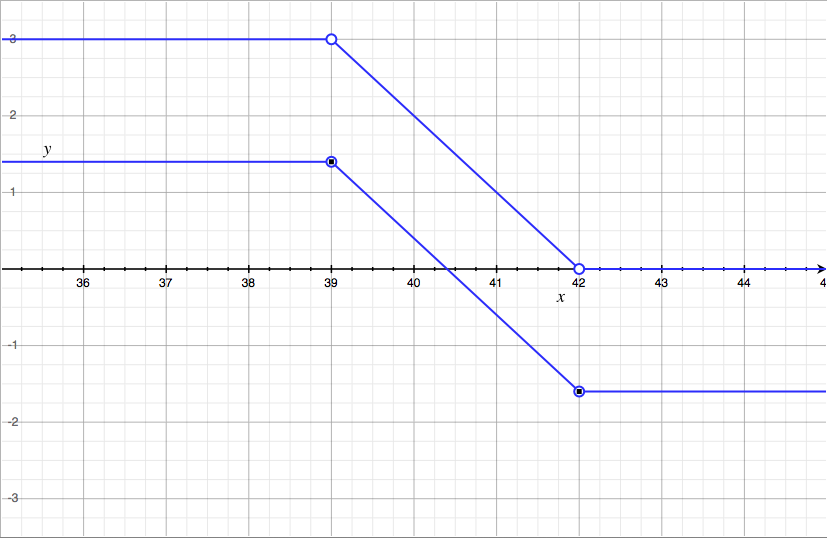
\includegraphics[scale=0.4]{4-1}
            \caption{The payoff diagram (hollow points) and the P\&L diagram (solid points) of 4(i)}
        \end{figure*} \\
        For $S(T) < 40.379874$ would the bear spread be profitable.
    \end{homeworkSection}
    \begin{homeworkSection}{(ii)}
        Synthesize: a short position in the 36 strike call and a long position in the 39 strike call. \\
        Payoff:
        \begin{equation}
            \begin{split}
                V(T) &= -\max\{S(T)-36,0\} + \max\{S(T)-39,0\} \\
                &=
                \begin{cases}
                    0, &\text{ if }S(T)\le36\\
                    36-S(T), &\text{ if }36<S(T)<\le39\\
                    -3, &\text{ if }39<S(T) 
                \end{cases}
            \end{split}
        \end{equation}
        P\&L:
        \begin{equation}
            \begin{split}
                P\&L(T) &= V(T) + (5.5 - 3.5)e^(rT) \\
                &=
                \begin{cases}
                    2.025157, &\text{ if }S(T)\le36\\
                    38.025156-S(T), &\text{ if }36<S(T)\le39\\
                    -0.974843, &\text{ if }39<S(T) 
                \end{cases}
            \end{split}
        \end{equation}
        \begin{figure*}[ht] \centering
            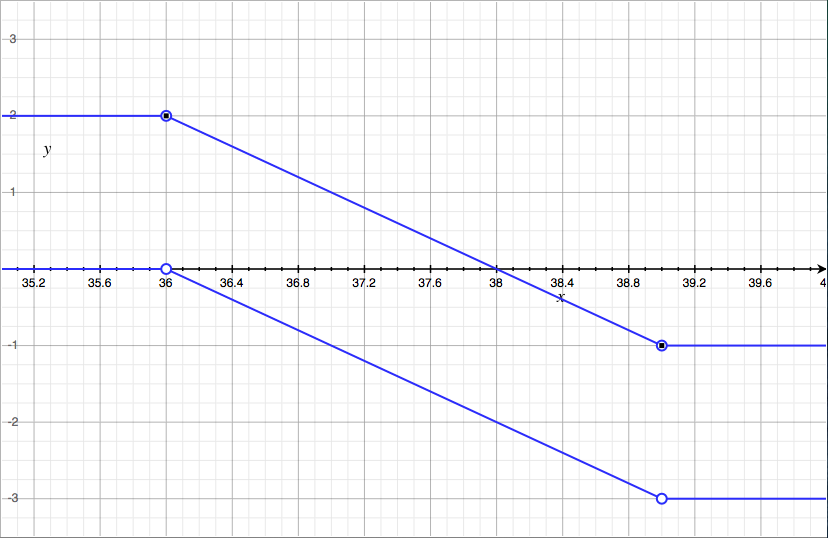
\includegraphics[scale=0.4]{4-2}
            \caption{The payoff diagram (hollow points) and the P\&L diagram (solid points) of 4(iii)}
        \end{figure*} \\
        For $S(T) < 38.025156$ would the bear spread be profitable.
    \end{homeworkSection}
    \begin{homeworkSection}{(iii)}
        Synthesize: a long position in one unit of the 36 strike call, a short position in two units of the 39 strike call and a long position in one unit of the 42 strike call \\
        Payoff:
        \begin{equation}
            \begin{split}
                V(T) &= \max\{S(T)-36,0\} - 2\max\{S(T)-39,0\} + \max\{S(T)-42,0\} \\
                &= 
                \begin{cases}
                    0, &\text{ if }S(T)\le36\\
                    S(T)-36, &\text{ if }36<S(T)\le39\\
                    42-S(T), &\text{ if }39<S(T)\le42\\
                    0, &\text{ if }42<S(T)
                \end{cases}
            \end{split}
        \end{equation}
        P\&L:
        \begin{equation}
            \begin{split}
                P\&L(T) &= V(T)-5.5+2\times3.5-2.5 \\
                &=
                \begin{cases}
                    -1.012578, &\text{ if }S(T)\le36\\
                    S(T)-37.012578, &\text{ if }36<S(T)\le39\\
                    40.987422-S(T), &\text{ if }39<S(T)\le42\\
                    -1.012578, &\text{ if }42<S(T)
                \end{cases}
            \end{split}
        \end{equation}
        \begin{figure*}[ht] \centering
            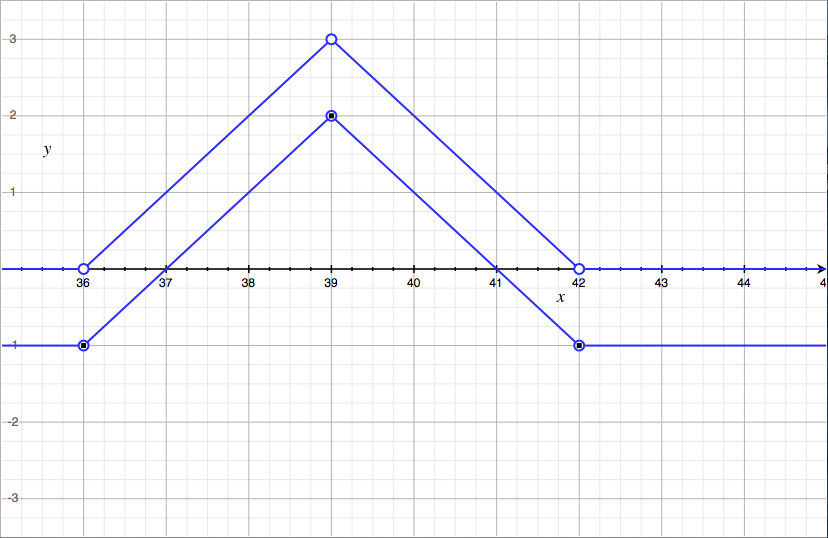
\includegraphics[scale=0.4]{4-3}
            \caption{The payoff diagram (hollow points) and the P\&L diagram (solid points) of 4(ii)}
        \end{figure*} \\
        For $37.012578 < S(T) < 40.987422$ would the butterfly spread be profitable.
    \end{homeworkSection}
    \begin{homeworkSection}{(iv)}
        A 36–42 strangle: a long position in the 36 strike put and a long position in the 42 strike call\\
        Payoff:
        \begin{equation}
            \begin{split}
                V(T) &= \max\{36-S(T),0\} + \max\{S(T)-42\} \\
                &=
                \begin{cases}
                    36-S(T), &\text{ if }S(T)<36\\
                    0, &\text{ if }36\le S(T)<42\\
                    S(T)-42, &\text{ if }42\le S(T)
                \end{cases}
            \end{split}
        \end{equation}
        P\&L:
        \begin{equation}
            \begin{split}
                P\&L(T) &= V(T)-(1.2+2.5)e^{rT} \\
                &=
                \begin{cases}
                    32.253460-S(T), &\text{ if }S(T)<36\\
                    -3.746540, &\text{ if }36\le S(T)<42\\
                    S(T)-45.746540, &\text{ if }42\le S(T)
                \end{cases}
            \end{split}
        \end{equation}
        \begin{figure*}[ht] \centering
            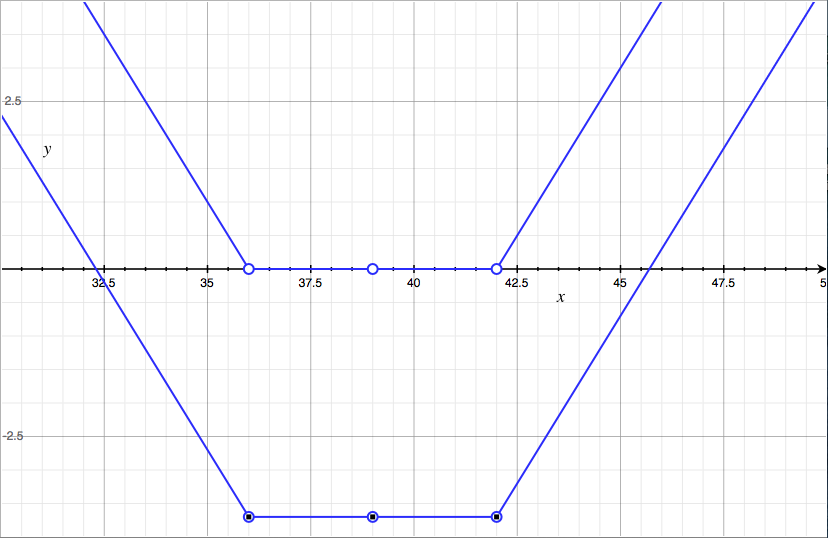
\includegraphics[scale=0.4]{4-4}
            \caption{The payoff diagram (hollow points) and the P\&L diagram (solid points) of a 36-42 strangle}
        \end{figure*} \\
        For $S(T) < 32.253460$ or $S(T > 45.746540$ would the strangle be profitable. \\

        A 39 straddle: a long position in th 39 strike put and a long position in the 39 strike call\\
        Payoff:
        \begin{equation}
            \begin{split}
                V(T) &= \max\{39-S(T),0\} + \max\{S(T)-39,0\} \\
                &=
                \begin{cases}
                    39-S(T), &\text{ if }S(T)\le39 \\
                    S(T)-39, &\text{ if }S(T)>39
                \end{cases}
            \end{split}
        \end{equation}
        P\&L:
        \begin{equation}
            \begin{split}
                P\&L(T) &= V(T) - (2.4 + 3.5)e^{rT} \\
                &=
                \begin{cases}
                    33.025787-S(T), &\text{ if }S(T)\le39\\
                    S(T)-44.974213, &\text{ if }S(T)>39
                \end{cases}
            \end{split}
        \end{equation}
        \begin{figure*}[ht] \centering
            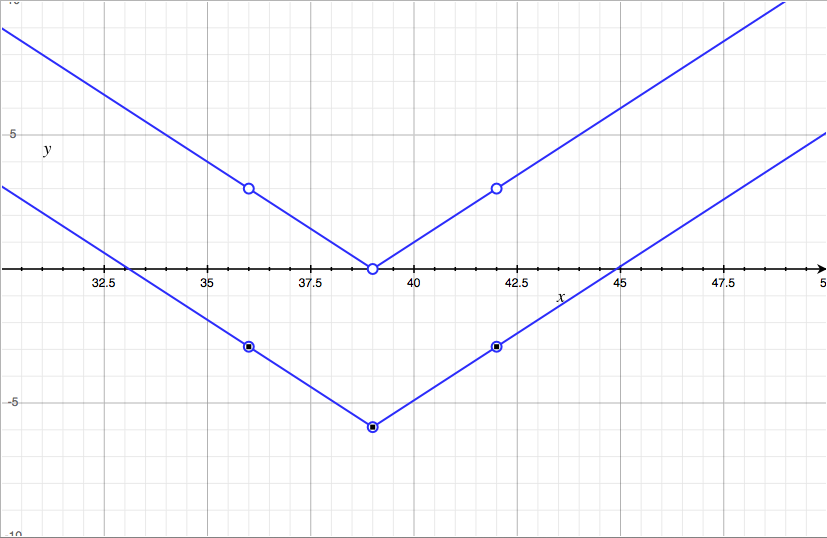
\includegraphics[scale=0.4]{4-5}
            \caption{The payoff diagram (hollow points) and the P\&L diagram (solid points) of a 39 straddle}
        \end{figure*} \\
        For $S(T)<33.025787$ or $S(T)>44.974213$ would the 39 straddle be profitable. \\

        A 36–42 collar: long the underlying, long a put option at strike price 36, short a call option at strike price 42 \\
        Payoff:
        \begin{equation}
            \begin{split}
                V(T) &= S(T)+\max\{36-S(T),0\}-\max\{S(T)-42,0\} \\
                &=
                \begin{cases}
                    36, &\text{ if }S(T)\le36\\
                    S(T), &\text{ if }36<S(T)\le42\\
                    42, &\text{ if }42<S(T)
                \end{cases}
            \end{split}
        \end{equation}
        P\&L:
        \begin{equation}
            \begin{split}
                P\&L(T) &= V(T) + (- 40 - 1.2 + 2.5)e^{rT} \\
                &=
                \begin{cases}
                    -3.186786, &\text{ if }S(T)\le36\\
                    S(T)-39.186786, &\text{ if }36<S(T)\le42\\
                    2.813214, &\text{ if }42<S(T)
                \end{cases}
            \end{split}
        \end{equation}
        \begin{figure*}[ht] \centering
            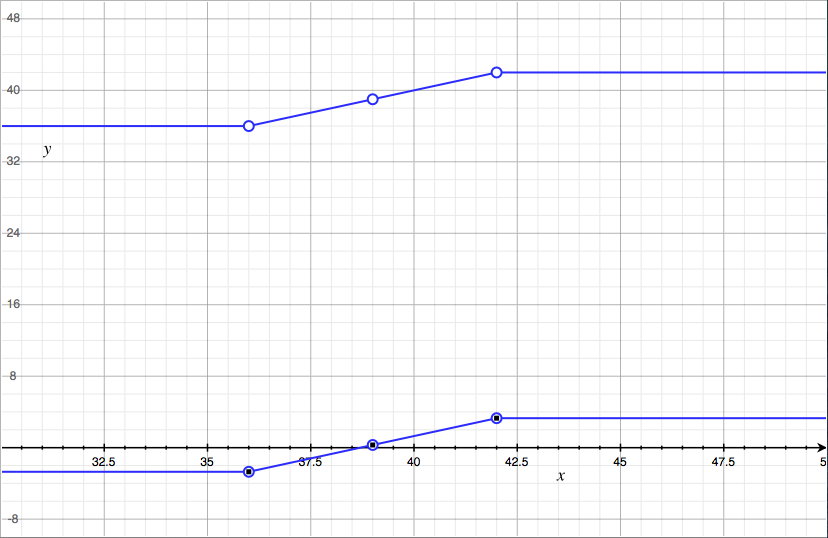
\includegraphics[scale=0.4]{4-6}
            \caption{The payoff diagram (hollow points) and the P\&L diagram (solid points) of a 36-42 collar}
        \end{figure*} \\
        For $S(T)>39.186786$ would the 36-42 collar be profitable. \\

        A 36–42 risk reversal: short a put option at strike price 36, long a call option at strike price 42 \\
        Payoff:
        \begin{equation}
            \begin{split}
                V(T) &= -\max\{36-S(T),0\} + \max\{S(T)-42,0\} \\
                &= 
                \begin{cases}
                    S(T)-36, &\text{ if }S(T)\le36\\
                    0, &\text{ if }36<S(T)\le42\\
                    S(T)-42, &\text{ if }42<S(T)
                \end{cases}
            \end{split}
        \end{equation}
        P\&L:
        \begin{equation}
            \begin{split}
                P\&L(T) &= V(T) + (1.2 - 2.5)e^{rT} \\
                &=
                \begin{cases}
                    S(T)-37.316352, &\text{ if }S(T)\le36\\
                    -1.316352, &\text{ if }36<S(T)\le42\\
                    S(T)-43.316352, &\text{ if }42<S(T)
                \end{cases}
            \end{split}
        \end{equation}
        \begin{figure*}[ht] \centering
            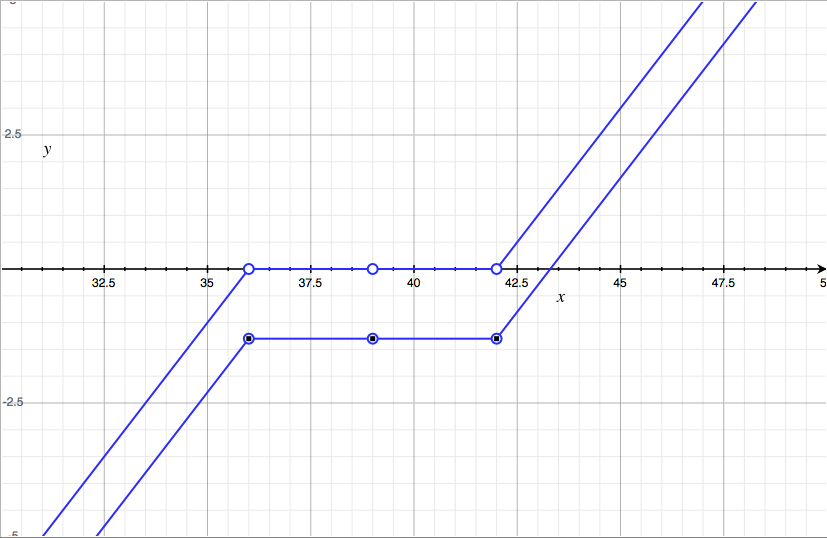
\includegraphics[scale=0.4]{4-7}
            \caption{The payoff diagram (hollow points) and the P\&L diagram (solid points) of a 36-42 risk reversal}
        \end{figure*} \\
        For $S(T) > 43.316352$ would the 36-42 risk reversal be profitable.
    \end{homeworkSection}
\end{homeworkProblem}

%----------------------------------------------------------------------------------------
%   PROBLEM 5
%----------------------------------------------------------------------------------------

\begin{homeworkProblem}
    \begin{homeworkSection}{(i)}
        To derive the maximum of $V(S)$, 
        \begin{equation}
            \begin{split}
                \frac{\partial V(S)}{\partial S} &= N(d) - \frac{\partial \max\{S-K,0\}}{S} \\
                &= 
                \begin{cases}
                    N(d)-1 < 0, &\text{ if }S>K \\
                    N(d) \ge 0, &\text{ if }S\le K
                \end{cases}
            \end{split}
        \end{equation}
        where 
        \begin{equation}
            d = \frac{ln(S/K)+(r+\sigma^2/2)(T-t)}{\sigma\sqrt{T-t}}
        \end{equation}
        Therefore the maximum value of $V(S)$ is obtained when $S=K$.
    \end{homeworkSection}
    \begin{homeworkSection}{(ii)}
        If $S \to \infty$,
        \begin{equation}
            d \to \infty, d_2 \to \infty \Rightarrow N(d) = N(d_2) = 1
        \end{equation}
        Therefore,
        \begin{equation}
            \begin{split}
                V(S) &= C_BS(S) - \max\{S-K,0\} \\
                &= (SN(d)-Ke^{-r(T-t)}N(d_2)) - (S-K) \\
                &\to (S-Ke^{-r(T-t)}) - (S-K) \\
                &= K(1-e^{-r(T-t)})
            \end{split}
        \end{equation}
        We also find from from part(i) that $V'(S) \to 0$ when $S \to \infty$, which indicates convergence, so we can conclude $V(S) \to K(1-e^{-r(T-t)})$.
    \end{homeworkSection}
    \begin{homeworkSection}{(iii)}
        This is a graph generated by following python code -
        \begin{lstlisting}
from math import *
from scipy.stats import norm
import numpy as np
import matplotlib.pyplot as plt

# Black Sholes Function
def BlackSholes(CallPutFlag,S,X,T,r,v):
    d1 = (log(S/X)+(r+v*v/2.)*T)/(v*sqrt(T))
    d2 = d1-v*sqrt(T)
    if CallPutFlag=='c':
        return S*norm.cdf(d1)-X*exp(-r*T)*norm.cdf(d2)
    else:
        return X*exp(-r*T)*norm.cdf(-d2)-S*norm.cdf(-d1)

def Premium(S):
    return BlackSholes(CallPutFlag='c',S=S,X=100.,T=0.5,r=0.05,v=0.3) - max(S-100.,0.)

x = np.linspace(50, 200)
y = [Premium(i) for i in x]
plt.plot(x, y, 'r', linewidth=2)

plt.savefig('5-3.pdf')
        \end{lstlisting}
        where I assumed strike as 100, maturity as 6 months, risk rate as 5\% and volatilty as 30\%.
        \begin{figure*}[ht] \centering
            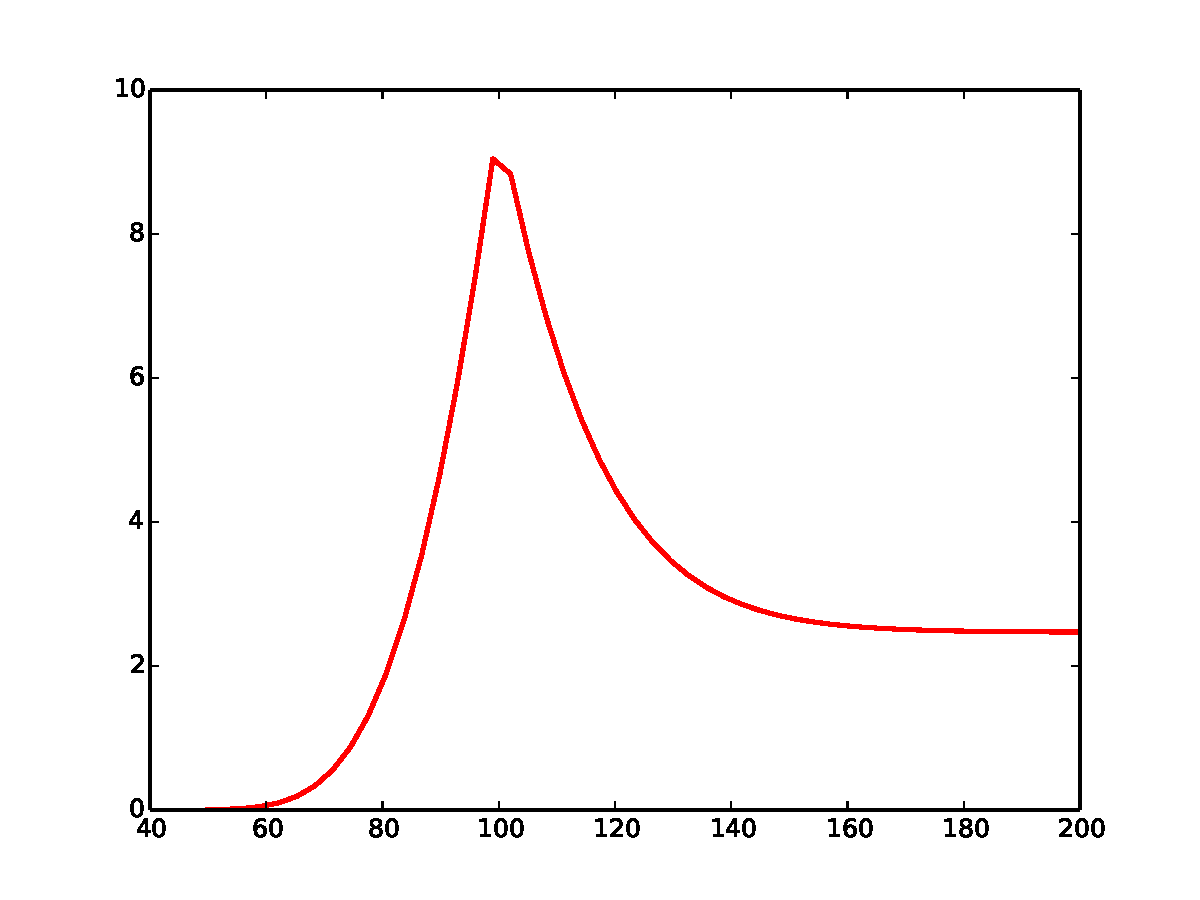
\includegraphics[scale=0.5]{5-3}
            \caption{Plot of $V(S)$ as a function of $S$}
        \end{figure*}
    \end{homeworkSection}
    \begin{homeworkSection}{(iv)}
        When it comes to an European put option, we will have the delta as
        \begin{equation}
            \begin{split}
                \frac{\partial V(S)}{\partial S} &= -N(-d) - \frac{\partial \max\{K-S,0\}}{S} \\
                &= 
                \begin{cases}
                    -N(-d)+1 > 0, &\text{ if }S<K \\
                    -N(-d) \le 0, &\text{ if }S\ge K
                \end{cases}
            \end{split}
        \end{equation}
        Therefore the maximum value of $V(S)$ is obtained when $S=K$. \\
        If $S \to \infty$,
        \begin{equation}
            d \to \infty, d_2 \to \infty \Rightarrow N(-d) = N(-d_2) = 0
        \end{equation}
        Therefore,
        \begin{equation}
            \begin{split}
                V(S) &= P_BS(S) - \max\{K-S,0\} \\
                &= (-SN(-d)+Ke^{-r(T-t)}N(-d_2)) - 0 \\
                &\to (0-0)-0 \\
                &= 0
            \end{split}
        \end{equation}
        If $S \to 0$,
        \begin{equation}
            d \to -\infty, d_2 \to -\infty \Rightarrow N(-d) = N(-d_2) = 1
        \end{equation}
        Therefore,
        \begin{equation}
            \begin{split}
                V(S) &= P_BS(S) - \max\{K-S,0\} \\
                &= (-SN(-d)+Ke^{-r(T-t)}N(-d_2)) - K \\
                &\to (0+Ke^{-r(T-t)})-K \\
                &= K(e^{-r(T-t)}-1)
            \end{split}
        \end{equation}
        The graph generated by similar python codes -
        \begin{figure*}[ht] \centering
            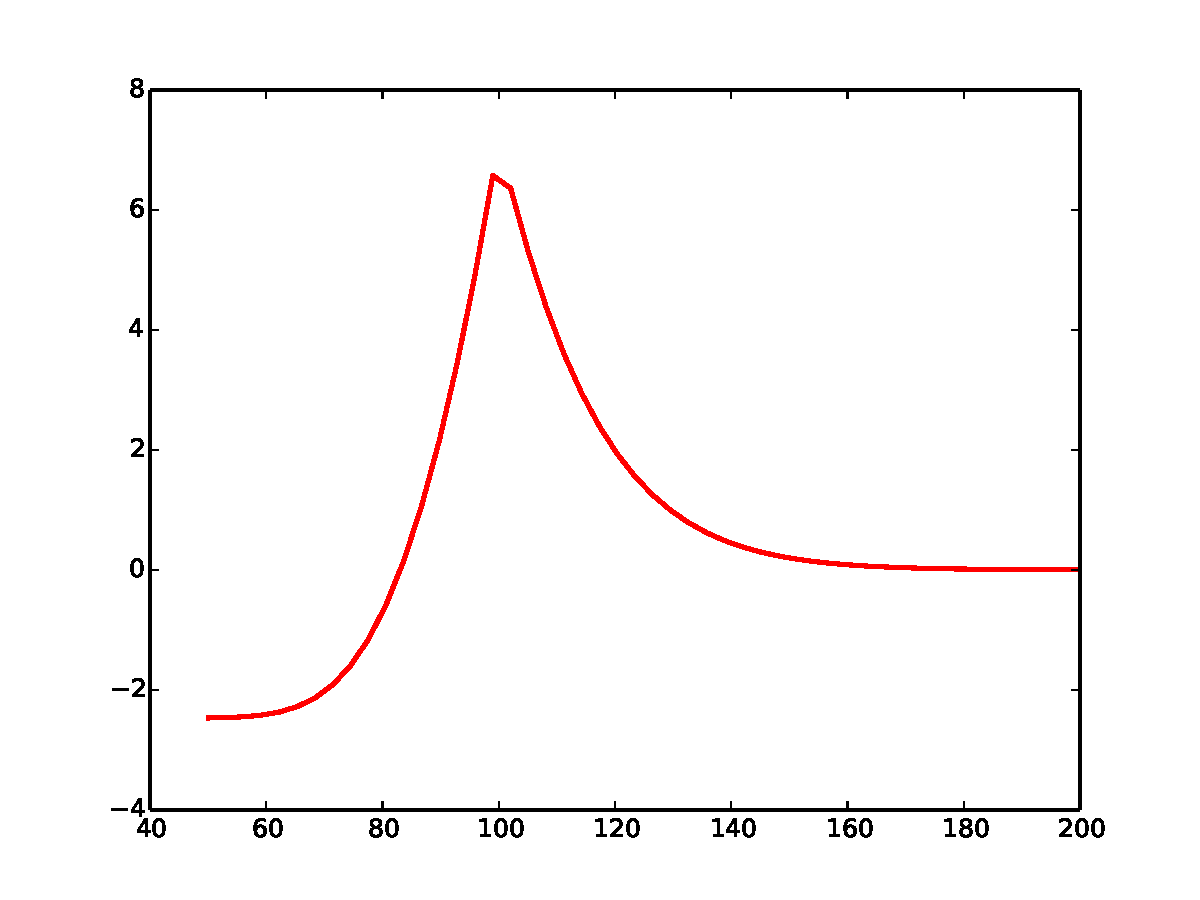
\includegraphics[scale=0.5]{5-4}
            \caption{Plot of $V(S)$ as a function of $S$}
        \end{figure*}
    \end{homeworkSection}
\end{homeworkProblem}

%----------------------------------------------------------------------------------------
%   PROBLEM 6
%----------------------------------------------------------------------------------------

\begin{homeworkProblem}
    \begin{homeworkSection}{(i)}
        The cash flow of the coupon bound is
        \begin{equation}
            \begin{split}
                v\_cash\_flow &= [1.75, 1.75, 1.75, 1.75, 101.75] \\
                t\_cash\_flow &= [1./12,7./12,13./12,19./12,25./12]
            \end{split}
        \end{equation}
        Given the risk–free zero rate curve, we are able to generate the value of the bond as
        \begin{equation}
            B = \sum_i v_ie^{-t_ir(0,t_i)} = 101.369304142
        \end{equation}
        The bond value can also be written as the expression of yield,
        \begin{equation}
            B = \sum_i v_ie^{-yt_i}
        \end{equation}
        We solved $y = 0.035126068375$.
    \end{homeworkSection}
    \begin{homeworkSection}{(ii)}
        Given the yield, the modified duration is
        \begin{equation}
            D = \frac{1}{B} \sum_i v_it_ie^{-t_iy} = 1.998752969544
        \end{equation}
        And the convexity is
        \begin{equation}
            C = \frac{1}{B} \sum_i v_it_i^2e^{-t_iy} = 4.115468941420
        \end{equation}
    \end{homeworkSection}
\end{homeworkProblem}

%----------------------------------------------------------------------------------------
%   PROBLEM 7
%----------------------------------------------------------------------------------------

\begin{homeworkProblem}
    \begin{homeworkSection}{(i)}
        The instantateous interest rate curve is
        \begin{equation}
            \begin{split}
                r_c(t) &= \frac{dr_c(0,t)t}{dt} \\
                &= t \frac{dr_c(0,t)}{dt} + r_c(0,t) \\
                &= 0.01t \times \frac{2+t}{2+2t} \times \frac{(2+t)-t}{(2+t)^2} + r_c(0,t) \\
                &= \frac{0.02t}{(2+2t)(2+t)} + 0.03 + 0.01\ln(1+\frac{t}{2+t})
            \end{split}
        \end{equation}
    \end{homeworkSection}
    \begin{homeworkSection}{(ii)}
        Since
        \begin{equation}
            (1+\frac{r_m(0,t)}{m})^m = \exp(r_c(0,t))
        \end{equation}
        then for annually compounded zero rate curve,
        \begin{equation}
            \begin{split}
                r_1(0,t) &= \exp(r_c(0,t)) - 1 \\
                &= \exp(0.03) * (1+\frac{t}{2+t})^{0.01} - 1 \\
                &= e^{0.03}(1+\frac{t}{2+t})^{0.01} - 1
            \end{split}
        \end{equation}
    \end{homeworkSection}
    \begin{homeworkSection}{(iii)}
        For semiannually compounded zero rate curve,
        \begin{equation}
            \begin{split}
                r_2(0,t) &= 2(\exp(\frac{r_c(0,t)}{2}) - 1) \\
                &= 2(\exp(0.015)*(1+\frac{t}{2+t})^{0.005} - 1) \\
                &= 2e^{0.015}(1+\frac{t}{2+t})^{0.005} - 2
            \end{split}
        \end{equation}
    \end{homeworkSection}
\end{homeworkProblem}

%----------------------------------------------------------------------------------------
%   PROBLEM 8
%----------------------------------------------------------------------------------------

\begin{homeworkProblem}
    \begin{homeworkSection}{(i)}
        Given the instantaneous rate curve r(t)
        \begin{equation}
            r(t) = \frac{0.05}{1+\exp(-(1+t)^2)}
        \end{equation}
        we can use simpson's rule to compute the 3 months, 9 months, 15 months and 21 months discount factors as
        \begin{equation}
            \begin{split}
                disc(3./12) = \exp(-\int_0^{3/12}{r(\tau)d\tau}) &= 0.990302 \\
                disc(9./12) = \exp(-\int_0^{9/12}{r(\tau)d\tau}) &= 0.968268 \\
                disc(15./12) = \exp(-\int_0^{15/12}{r(\tau)d\tau}) &= 0.944845 \\
                disc(21./12) = \exp(-\int_0^{21/12}{r(\tau)d\tau}) &= 0.92157243
            \end{split}
        \end{equation}
    \end{homeworkSection}
    \begin{homeworkSection}{(ii)}
        Cash flow of the 21 months year semiannual coupon bond with coupon rate 5\% is
        \begin{equation}
            \begin{split}
                v\_cash\_flow = [2.5, 2.5, 2.5, 102.5]
                t\_cash\_flow = [3./12, 9./12, 15./12, 21./12]
            \end{split}
        \end{equation}
        The price of the 21 months year semiannual coupon bond with coupon rate 5\% is
        \begin{equation}
            B = \sum_i {v_i disc(t_i)} = 101.719713273
        \end{equation}
    \end{homeworkSection}
\end{homeworkProblem}

%----------------------------------------------------------------------------------------
%   PROBLEM 9
%----------------------------------------------------------------------------------------

\begin{homeworkProblem}
    \begin{homeworkSection}{(i)}
        The cash flows of the fixed leg is
        \begin{equation}
            \begin{split}
                fixed\_cash\_flow &= [200000.0, 200000.0, 200000.0, 10200000.0] \\
                t &= [0.5, 1.0, 1.5, 2.0]
            \end{split}
        \end{equation}
        The cash flows of the floating leg is
        \begin{equation}
            \begin{split}
                Notional \times \frac{r(0, 0.5)}{2} &= 75000.0\\
                Notional \times \frac{r(0.5, 1.0)}{2} &= 112500.0\\
                Notional \times \frac{r(1.0, 1.5)}{2} &= 150000.0\\
                Notional \times \frac{r(1.5, 2.0)}{2} &= 10106250.0\\
            \end{split}
        \end{equation}
        where the units are dollars. Therefore the cash flows of the swap is
        \begin{equation}
            \begin{split}
                swap\_cash\_flow &= fixed\_cash\_flow - float\_cash\_flow \\
                &= [200000.0, 200000.0, 200000.0, 10200000.0] \\
                &- [75000.0, 112500.0, 150000.0, 10106250.0] \\
                &= [125000.00, 87500.00, 50000.00, 93750.00]
            \end{split}
        \end{equation}
        where the units are dollars and their corresponded time is $t = [0.5, 1.0, 1.5, 2.0]$.
    \end{homeworkSection}
    \begin{homeworkSection}{(ii)}
        At $t_1=4./12$, the value of the fixed rate bond underlying the swap
        \begin{equation}
            \begin{split}
                v_{fixed} = \sum_{i} fixed\_cash\_flow[i] \times (1+0.5r(t_1,t_i))^{-2(t_i-t)} = 38,884,742.17
            \end{split}
        \end{equation}
        dollars. For the floating leg, the next payment (2 months later) is decided 4 months ago using zero rate curve at time 0, that is
        \begin{equation}
            Notional \times \frac{r_0(0,0.5)}{2} = 75,000
        \end{equation}
        million dollars, where $r_0(0,0.5)$ is 6-month LIBOR observed 4 months ago; $0.075$ million dollars is the next interest rate payment that will be paid 2 months from now. The floating rate bond will be worth its par value of $10.$ million dollars, immediately after the next interest payment of $0.075$. \\
        The value of the floating rate bond underlying the swap is
        \begin{equation}
            v_{float} = (75,000 + 10,000,000) (1+\frac{r(0, 2./12)}{2})^{-\frac{2./12}{0.5}} = 10,031,991.35
        \end{equation}
        Therefore the value of the swap is
        \begin{equation}
            v_{swap} = v_{fixed} - v_{float} = 28852750.82
        \end{equation}
    \end{homeworkSection}
\end{homeworkProblem}

%----------------------------------------------------------------------------------------
%   PROBLEM 10
%----------------------------------------------------------------------------------------

\begin{homeworkProblem}
    According the question, we have
    \begin{equation}
        2.5e^{-4.5\%(.5)} + 2.5e^{-4.5\%(1.0)} + 102.5e^{-1.5R} = 100.
    \end{equation}
    Therefore the 18-months LIBOR rate is
    \begin{equation}
        R = 0.049495980179 \approx 4.949598\%
    \end{equation}
\end{homeworkProblem}

%----------------------------------------------------------------------------------------
%   PROBLEM 11
%----------------------------------------------------------------------------------------

\begin{homeworkProblem}
    The value of the fixed rate bond underlying the swap is
    \begin{equation}
        2.5e^{-0.04 \times \frac{4}{12}} + 2.5e^{-0.04 \times \frac{10}{12}} + 102.5e^{-0.04 \times \frac{16}{12}} = 102.061481851
    \end{equation}
    The value of the floating rate bond underlying the swap is
    \begin{equation}
        (2.5 + 100)e^{-0.04 \times \frac{4}{12}} = 101.142404085
    \end{equation}
    $2.5$ equals $.5 \times 5\% \times 100$, where $5\%$ is 6-month LIBOR observed 2 months ago; $2.5$ is the next interest rate payment that will be paid 4 months from now. The floating rate bond will be worth its par value of $100$ immediately after the next interest payment of $2.5$. \\
    Since the firm in question receives floating and pays fixed, the value of the swap is
    \begin{equation}
        101.142404085 - 102.061481851  = -0.919077766058
    \end{equation}
    where the unit is million dollars, so it's $-919077.77$ dollars.
\end{homeworkProblem}

%----------------------------------------------------------------------------------------
%   PROBLEM 12
%----------------------------------------------------------------------------------------

\begin{homeworkProblem}
    \begin{homeworkSection}{(i)}
        The value of a put options with strike price 40 and maturity of three months, on a non dividend paying stock with lognormal distribution with volatility 30\% is
        \begin{equation}
           P = e^{-r\tau}KN(-d_2)-Se^{-q\tau}N(-d) = 5.4075696734
        \end{equation}
        Therefore the value of the portfolio is
        \begin{equation}
            V(\Pi) = 2000P + 400S + 10000 = 34815.1393468 \approx 34815.14
        \end{equation}
    \end{homeworkSection}
    \begin{homeworkSection}{(ii)}
        Delta of the current portfolio is
        \begin{equation}
            \Delta(\Pi) = 2000\Delta{\Pi} + 400 = -1165.71252025 
        \end{equation}
        To make the portfolio Delta-neutral, we have to long 1166 shares of the same stock.
    \end{homeworkSection}
    \begin{homeworkSection}{(iii)}
\begin{table}[ht]
\centering
\begin{tabular}{l|lll}
            & Options Position & Asset Position & Cash Position \\ \hline
Week 0 - AH: & 2000P=10815.14    & 1566S=54810.00        & -30810.00      \\
Week 1 - BH: & 2000P=4573.58     & 1566S=62640.00        & -30821.74      \\
Week 1 - AH: & 2000P=4573.58     & 914S=36560.00         & -4741.74       \\
Week 2 - BH: & 2000P=9306.89     & 914S=32904.00         & -4743.54       \\
Week 2 - AH: & 2000P=9306.89     & 1448S=52128.00        & -23967.54      \\
Week 3 - BH: & 2000P=15948.01    & 1448S=46336.00        & -23976.67      \\
Week 3 - AH: & 2000P=15948.01    & 1832S=58624.00        & -36264.67      \\
Week 4 - BH: & 2000P=7921.98    & 1832S=67784.00         & -36278.48      \\
Week 4 - AH: & 2000P=7921.98    & 1319S=48803.00         & -17297.48           
\end{tabular}
\end{table}

\begin{table}[ht]
\centering
\begin{tabular}{l|l}
       & Hedging Action \\ \hline
Week 1 & sell 652 shares of u.a  \\
Week 2 & buy 534 shares of u.a  \\
Week 3 & buy 384 shares of u.a  \\
Week 4 & sell 513 shares of u.a
\end{tabular}
\end{table}
    \end{homeworkSection}
\end{homeworkProblem}

%----------------------------------------------------------------------------------------
%   PROBLEM 13
%----------------------------------------------------------------------------------------

\newpage
\begin{homeworkProblem}
    \begin{homeworkSection}{(i)}
        Delta of current portfolio is
        \begin{equation}
            \Delta(\Pi) = 1000\Delta(C) + 600\Delta(P) = 182.729986558
        \end{equation}
        To delta hedge, we need to sell 183 shares of underlying asset, which will create cash
        \begin{equation}
            c_1 = 183S = \$9150.0
        \end{equation}
    \end{homeworkSection}
    \begin{homeworkSection}{(ii)}
        Suppose we will long $x_1$ units of the underlying asset and $x_2$ units of the 9-month ATM call to Delta hedge and Gamma hedge,
        \begin{equation}
            \begin{split}
                \Delta(\Pi) &= 1000\Delta(C) + 600\Delta(P) + x_1 + x_2\Delta(C_{ATM}) = 0 \\
                \Gamma(\Pi) &= 1000\Gamma(C) + 600\Gamma(P) + x_2\Gamma(C_{ATM}) = 0
            \end{split}
        \end{equation}
        where
        \begin{equation}
            \begin{split}
                \Delta(C) &= e^{-q\tau}N(d) = 0.294224765689 \\
                \Delta(P) &= -e^{-q\tau}N(-d) = -0.185824631885 \\
                \Delta(C_{ATM}) &= 0.560287227854 \\
                \Gamma(C) &= e^{-q \tau} \frac{N(d)}{S\sigma\sqrt{\tau}} = 0.0484733742912 \\
                \Gamma(P) &= e^{-q \tau} \frac{N(d)}{S\sigma\sqrt{\tau}} = 0.0377099419132 \\
                \Gamma(C_{ATM}) &= 0.0447044338962
            \end{split}
        \end{equation}
        Therefore we can derive 
        \begin{equation}
            \begin{split}
                x_1 &= 708.36846442 \approx 708 \\
                x_2 &= -1590.43149062 \approx -1590
            \end{split}
        \end{equation}
        That is, we need to long 708 units of the underlying asset and short 1590 units of the 9-month ATM call, this will create cash
        \begin{equation}
            c_2 = -x_1S - x_2C_{ATM} = -29449.1790844
        \end{equation}
        which means cost 29449.18 dollars.
    \end{homeworkSection}
    \begin{homeworkSection}{(iii)}
        For the three portfolios, the original values are
        \begin{equation}
            \begin{split}
                V(\Pi_0) &= 1000C + 600P = 1687.0368332 \\
                V(\Pi_1) &= 1000C + 600P - 183S + c_1 = 1687.0368332 \\
                V(\Pi_2) &= 1000C + 600P + 708S - 1590C_{ATM} + c_2 = 1687.0368332               
            \end{split}
        \end{equation}
        After $1.$ day ($\Delta t = 1./252$ year) the asset price jumps at 54, and the volatility of the asset also jumps to 0.3, the values of the three portfolios become
        \begin{equation}
            \begin{split}
                V(\Pi_0) &= 1000C + 600P = 4917.05250929 \\
                V(\Pi_1) &= 1000C + 600P - 183Se^{q\Delta t} + c_1e^{r\Delta(t)} = 4185.70012914 \\
                V(\Pi_2) &= 1000C + 600P + 708Se^{q\Delta t} - 1590C_{ATM} + c_2e^{r\Delta t} = 1085.56128968                   
            \end{split}
        \end{equation}
        Therefore the change of the value is
        \begin{equation}
            \begin{split}
                \Delta V(\Pi_0) &= 3230.01567609 \\
                \Delta V(\Pi_1) &= 2498.66329594 \\
                \Delta V(\Pi_2) &= -601.475543525                
            \end{split}
        \end{equation}
    \end{homeworkSection}
\end{homeworkProblem}

%----------------------------------------------------------------------------------------
%   PROBLEM 14
%----------------------------------------------------------------------------------------

\begin{homeworkProblem}
    Recall the Black-Scholes formula
    \begin{equation}
        C = Se^{-q(T-t)}N(d) - Ke^{-r(T-t)}N(d_2)
    \end{equation}
    and the 'magic of Greeks computations', i.e., the fact that
    \begin{equation}
        Se^{-q(T-t)}N'(d) = Ke^{-r(T-t)}N'(d_2)
    \end{equation}
    Then,
    \begin{equation}
        \begin{split}
            \frac{\partial C}{\partial K} &= Se^{-q(T-t)}N'(d) \frac{\partial d}{\partial K} - Ke^{-r(T-t)}N'(d_2) \frac{\partial d_2}{\partial K} - e^{-r(T-t)}N(d_2) \\
            &= Se^{-q(T-t)}N'(d) (\frac{\partial d}{\partial K} - \frac{\partial d_2}{\partial K}) - e^{-r(T-t)}N(d_2) \\
            &= -e^{-r(T-t)}N(d_2)
        \end{split}
    \end{equation}
    since $d - d_2 = \sigma \sqrt{T-t}$ and therefore
    \begin{equation}
        \frac{\partial d}{\partial d_K} - \frac{\partial d_2}{\partial d_K} = 0
    \end{equation}
    By continously differentiating with respect to $K$, we obtain that
    \begin{equation}
        \begin{split}
            \frac{\partial^2 C}{\partial K^2} &= -e^{-r(T-t)}N'(d_2) \frac{\partial d_2}{\partial K} \\
            &= -e^{-r(T-t)} \frac{1}{\sqrt{2\pi}}e^{d_2^2/2} (-\frac{1}{K\sigma\sqrt{T-t}}) \\
            &= \frac{1}{K\sigma\sqrt{2\pi(T-t)}} \exp(-r(T-t)-\frac{d_2^2}{2})
        \end{split}
    \end{equation}
    By differentiating with respect to $K$ the Put-Call parity formula
    \begin{equation}
        P + Se^{-q(T-t)} - C = Ke^{-r(T-t)}
    \end{equation}
    and using former equations, we find that
    \begin{equation}
        \frac{\partial P}{\partial K} = \frac{\partial C}{\partial K} + e^{-r(T-t)} = e^{-r(T-t)}N(-d_2)
    \end{equation}
    By differentiating twice respect to $K$ the Put-Call parity and using former equations, we conclude that
    \begin{equation}
        \frac{\partial^2 P}{\partial K^2} = \frac{\partial^2 C}{\partial K^2} = \frac{1}{K\sigma\sqrt{2\pi(T-t)}} \exp(-r(T-t)-\frac{d_2^2}{2})
    \end{equation}
\end{homeworkProblem}

%----------------------------------------------------------------------------------------
%   PROBLEM 15
%----------------------------------------------------------------------------------------

\begin{homeworkProblem}
    The following python will be able to generate the Deltas and Gammas with different strikes
    \begin{lstlisting}
from mibian import *

spotPrice = 50.
dividendsYield = 0.02 * spotPrice
volatility = 0.3 * 100
riskFreeRate = 0.02 * 100
ls_strike = [40.,45.,50.,55.,60.]
maturity = 3./12 * 365

for f_strike in ls_strike:
    option = Me([spotPrice, f_strike, riskFreeRate, dividendsYield, maturity], volatility=volatility)
    straddleDelta = option.putDelta + option.callDelta
    straddleGamma = option.gamma + option.gamma
    print f_strike, "straddleDelta:", round(straddleDelta,6)
    print f_strike, "straddleGamma:", round(straddleGamma,6)
    \end{lstlisting}
    The output is
    \begin{lstlisting}
40.0 straddleDelta: 0.877461
40.0 straddleGamma: 0.031223
45.0 straddleDelta: 0.560271
45.0 straddleGamma: 0.078248
50.0 straddleDelta: 0.059487
50.0 straddleGamma: 0.105557
55.0 straddleDelta: -0.422676
55.0 straddleGamma: 0.090472
60.0 straddleDelta: -0.742192
60.0 straddleGamma: 0.055242
    \end{lstlisting}
\end{homeworkProblem}

%----------------------------------------------------------------------------------------
%   PROBLEM 16
%----------------------------------------------------------------------------------------

\begin{homeworkProblem}
    \begin{homeworkSection}{AoN Call}
        This pays out one unit of asset if the spot is above the strike at maturity. Its value now is given by,
        \begin{equation}
            \begin{split}
                C &= e^{-r(T-t)}E[S_TI_{S_T>K}] \\
                &= e^{-r(T-t)} \int_{Z_0}^{\infty}Se^z\phi(z)dz \\
                &= SN(d)
            \end{split}
        \end{equation}
        where
        \begin{equation}
            d = \frac{\ln\frac{S}{K} + (r+\sigma^{2}/2)(T-t)}{\sigma\sqrt{T-t}}
        \end{equation}
        which give us the following PDEs
        \begin{equation}
            \begin{split}
                \frac{\partial d}{\partial S} &= \frac{1}{S\sigma \sqrt{T-t}} \\
                \frac{\partial d}{\partial t} &= \frac{d}{2(T-t)} - \frac{r+\sigma^2/2}{\sigma\sqrt{T-t}} \\
                \frac{\partial d}{\partial r} &= \frac{\sqrt{T-t}}{\sigma} \\
                \frac{\partial d}{\partial \sigma} &= \sqrt{T-t} - \sigma d
            \end{split}
        \end{equation}
        Delta:
        \begin{equation}
            \begin{split}
                \Delta(C) &= \frac{\partial C}{\partial S} \\
                &= N(d) + SN'(d)\frac{\partial d}{\partial S} \\
                &= N(d) + S(\frac{1}{\sqrt{2\pi}}e^{-d^2/2}) (\frac{1}{\sigma\sqrt{T-t}} \frac{K}{S} \frac{1}{K}) \\
                &= N(d) + \frac{e^{-d^2/2}}{\sigma\sqrt{2\pi (T-t)}} \\
                &= N(d) + \frac{1}{\sigma\sqrt{T-t}}N'(d)
            \end{split}
        \end{equation}
        Gamma:
        \begin{equation}
            \begin{split}
                \Gamma(C) &= \frac{\partial \Delta(C)}{\partial S} \\
                &= N'(d)\frac{\partial d}{\partial S} + \frac{e^{-d^2/2}}{\sigma\sqrt{2\pi (T-t)}} (-d) \frac{\partial d}{\partial S} \\
                &= \frac{e^{-d^2/2}}{\sigma\sqrt{2\pi (T-t)}S} (1-\frac{d}{\sigma\sqrt{T-t}}) \\
                &= \frac{N'(d)}{\sigma S \sqrt{T-t}} [1-\frac{d}{\sigma\sqrt{T-t}}]              
            \end{split}
        \end{equation}
        Vega:
        \begin{equation}
            \begin{split}
                Vege(C) &= \frac{\partial C}{\partial \sigma} \\
                &= N'(d) \frac{\partial d}{\partial \sigma} \\
                &= N'(d) \frac{\sigma (T-t) - (\ln\frac{S}{K} + (r+\sigma^{2}/2)(T-t))\sqrt{T-t}}{\sigma^2(T-t)}  \\
                &= S(\frac{1}{\sqrt{2\pi}}e^{-d^2/2}) (\frac{\sigma \sqrt{T-t} - (\ln\frac{S}{K} + (r+\sigma^{2}/2)(T-t))}{\sigma^2\sqrt{T-t}}) \\
                &= S(\sqrt{T-t} - \sigma d)N'(d)      
            \end{split}
        \end{equation}
        Theta:
        \begin{equation}
            Theta(C) = SN'(d)\frac{d}{2(T-t)} - \frac{r+\frac{\sigma^2}{2}}{\sigma\sqrt{T-t}}
        \end{equation}
        where $N'(d)$ is the density function of the standard normal distribution and 
        \begin{equation}
            N'(x) = \frac{1}{\sqrt{2\pi}}e^{-\frac{x^2}{2}}
        \end{equation}
    \end{homeworkSection}
    \begin{homeworkSection}{AoN Put}
        Given the definitions of an asset-or-nothing call and put option and referring to the calculated price of the call option the put-call parity gives us the price of the put option as follows:
        \begin{equation}
            \begin{split}
                P &= S − C \\
                &= S - SN(d) \\
                &= S(1-N(d)) \\
                &= SN(-d)
            \end{split}
        \end{equation}
        Below are the conclusion of greeks calculated in similar ways:
        \begin{equation}
            \begin{split}
                \Delta(P) &= N(-d) - \sqrt{1}{\sigma\sqrt{T-t}}N'(-d) \\
                \Gamma(P) &= \Gamma(C_{AoN}) \\
                Vega(P) &= -S(\sqrt{T-t} - \sigma d) N'(-d) \\
                Theta(P) &= -S\frac{d}{2(T-t)} - \frac{r+\sigma^2/2}{\sigma\sqrt{T-t}}N'(-d)
            \end{split}
        \end{equation}
    \end{homeworkSection}
    \begin{homeworkSection}{CoN Call}
        If the asset price at maturity is higher than the strike, payoff is B else it is zero. This is also called a ‘bet’. This is simple to price because it is the probability of receiving B at maturity, discounted to today
        \begin{equation}
            C = e^{-r(T-t)}BN(d_2)
        \end{equation}
        where
        \begin{equation}
            d_2 = \frac{\ln\frac{S}{K} + (r-\sigma^{2}/2)(T-t)}{\sigma\sqrt{T-t}}
        \end{equation}
        Below are the conclusion of greeks calculated:
        \begin{equation}
            \begin{split}
                \Delta(C) &= B\frac{e^{-r(T-t)}N'(d_2)}{\sigma S \sqrt{T-t}} \\
                \Gamma(C) &= -e^{-r(T-t)}B\frac{d_1N'(d_2)}{\sigma^2S^2(T-t)} \\
                Vega(C) &= -e^{-r(T-t)}B\frac{N'(d_2)d_1}{\sigma} \\
                Theta(C) &= re^{-r(T-t)}BN(d_2) + e^{-r(T-t)}BN'(d_2)(\frac{d_1}{2(T-t)}-\frac{r}{\sigma\sqrt{T-t}})
            \end{split}
        \end{equation}
    \end{homeworkSection}
    \begin{homeworkSection}{CoN Put}
        Through put-call parity,
        \begin{equation}
            P = e^{-r(T-t)}B(1-N(d_2))
        \end{equation}
        Below are the conclusion of greeks calculated:
        \begin{equation}
            \begin{split}
                \Delta(P) &= -\Delta(C_{CoN}) \\
                \Gamma(P) &= \Gamma(C_{CoN}) \\
                Vega(P) &= Vega(C_{CoN}) \\
                Theta(C) &= re^{-r(T-t)}B(1-N(d_2)) - e^{-r(T-t)}BN'(d_2)(\frac{d_1}{2(T-t)}-\frac{r}{\sigma\sqrt{T-t}})
            \end{split}
        \end{equation}
    \end{homeworkSection}
\end{homeworkProblem}

%----------------------------------------------------------------------------------------
%   PROBLEM 17
%----------------------------------------------------------------------------------------

\begin{homeworkProblem}
    If using python, there are implemented libraries for newton's method and black-scholes pricing, therefore to realize the problem in the question is quite simple.
    \begin{lstlisting}
from scipy.optimize import newton
from mibian import *

def func(strike):
    spotPrice = 50.
    riskFreeRate = 0.02 * 100
    dividendsYield = 0.02 * spotPrice
    maturity = 3./12 * 365
    volatility = 0.3 * 100
    option = Me([spotPrice, strike, riskFreeRate, dividendsYield, maturity], volatility=volatility)
    return option.callDelta - 0.5

print newton(func=func, x0=spotPrice)
    \end{lstlisting}
    But if this problem requires my own implementation for newton's method, see follows.
    \begin{lstlisting}
def derivative(f):
    def compute(x, dx):
        return (f(x+dx) - f(x))/dx
    return compute

def newton(func, x0):
    dx=1e-6
    tolerance=1e-6
    df = derivative(f)
    while True:
        x1 = x - f(x)/df(x, dx)
        t = abs(x1 - x)
        if t < tolerance:
            break
        x = x1
    \end{lstlisting}
\end{homeworkProblem}

%----------------------------------------------------------------------------------------
%   PROBLEM 18
%----------------------------------------------------------------------------------------

\begin{homeworkProblem}
    Following is the python code to derive implied volatility using the secant method with initial guesses $x_0 = 0.5$ and $x_1 = 0.501$, and Newton’s method with initial guess $0.5$.
    \begin{lstlisting}
from scipy.optimize import newton
from scipy.optimize import secant
from mibian import *

def func(implied_volatility):
    spotPrice = 30.
    strike = 27.
    riskFreeRate = 0.04 * 100
    dividendsYield = 0.01 * spotPrice
    maturity = 7./12 * 365
    option = Me([spotPrice, strike, riskFreeRate, dividendsYield, maturity], volatility=implied_volatility)
    return option.callPrice - 4.5

print newton(func=func, x0=0.5)
print secant(func=func, x0=0.5, x1=0.501)
    \end{lstlisting}
    Both methods return the implied volatility as $28.0090064420\%$, or $0.280090064420$.
\end{homeworkProblem}

%----------------------------------------------------------------------------------------
%   PROBLEM 19
%----------------------------------------------------------------------------------------

\begin{homeworkProblem}
    \begin{homeworkSection}{(i)}
        Python code to compute the implied volatility using the bisection method, the secant method, and Newton’s method.
        \begin{lstlisting}
from scipy.optimize import bisect
from scipy.optimize import newton
from scipy.optimize import secant
from mibian import *

def func(implied_volatility):
    spotPrice = 40.
    strike = 40.
    riskFreeRate = 0.025 * 100
    dividendsYield = 0.01 * spotPrice
    maturity = 5./12 * 365
    option = Me([spotPrice, strike, riskFreeRate, dividendsYield, maturity], volatility=implied_volatility)
    return option.callPrice - 2.75

print bisect(func, 0.01, 100)
print newton(func, 50)
print secant(func, 50, 49)
        \end{lstlisting}
        All three methods return the same answer $25.6903172365\%$, or $0.256903172365$.
    \end{homeworkSection}
    \begin{homeworkSection}{(ii)}
        \begin{equation}
            \sigma_{imp,approx} = \frac{\sqrt{2\pi}}{S\sqrt{T}} \frac{C-\frac{(r-q)T}{2}S}{1-\frac{(r+q)T}{2}} = 0.256710246571
        \end{equation}
    \end{homeworkSection}
    Therefore the relative error is
        \begin{equation}
            \frac{|\sigma_{imp,approx} - \sigma_{imp}|}{\sigma_{imp}} = 0.000750966958487 \approx 0.000750966958
        \end{equation}
\end{homeworkProblem}

%----------------------------------------------------------------------------------------
%   PROBLEM 20
%----------------------------------------------------------------------------------------

\begin{homeworkProblem}
    In other words, this is to compute
    \begin{equation}
        V(0) = e^{-rT} E_{RN}[\max(\ln(\frac{S(T)}{K}),0)]
    \end{equation}
    Recall that
    \begin{equation}
        S(T) = S(0)\exp((r-\sigma^2/2)T+\sigma\sqrt{T}Z)
    \end{equation}
    And note that
    \begin{equation}
        S(T) \ge K \Rightarrow Z \ge \frac{\ln(K/S(0))-(r-\sigma^2/2)T}{\sigma\sqrt{T}} = -d_2
    \end{equation}
    Then,
    \begin{equation}
        \begin{split}
            V(0) &= e^{-rT} \frac{1}{\sqrt{2\pi}} \int_{-d_2}^{\infty} \ln(\frac{S(T)}{K})e^{-x^2/2}dx \\
            &= e^{-rT} \frac{1}{\sqrt{2\pi}} \int_{-d_2}^{\infty} \ln(\frac{S(0)\exp((r-\sigma^2/2)T+\sigma\sqrt{T}x)}{K})e^{-x^2/2}dx \\
            &= e^{-rT} \frac{1}{\sqrt{2\pi}} \int_{-d_2}^{\infty} [\ln\frac{S(0)}{K}+(r-\sigma^2/2)T]e^{-x^2/2} + \sigma\sqrt{T}xe^{-x^2/2} dx \\
            &= e^{-rT}[\ln\frac{S(0)}{K}+(r-\sigma^2/2)T]N(d_2) + \frac{\sigma\sqrt{T}e^{-rT-d_2^2/2}}{\sqrt{2\pi}}
        \end{split}
    \end{equation}
\end{homeworkProblem}

\end{document}